%%
%% This is file `hustreport-zh-example.tex',
%% generated with the docstrip utility.
%%
%% The original source files were:
%%
%% hustreport.dtx  (with options: `example-zh')
%% 
%% This is a generated file.
%% 
%% Copyright (C) 2013-2014 by Xu Cheng <xucheng@me.com>
%%               2014-2016 by hust-latex <https://github.com/hust-latex>
%% 
%% This work may be distributed and/or modified under the
%% conditions of the LaTeX Project Public License, either version 1.3
%% of this license or (at your option) any later version.
%% The latest version of this license is in
%%   http://www.latex-project.org/lppl.txt
%% and version 1.3 or later is part of all distributions of LaTeX
%% version 2005/12/01 or later.
%% 
%% This work has the LPPL maintenance status `maintained'.
%% 
%% The Current Maintainer of this work is hust-latex Organization.
%% 
%% This work consists of the files hustreport.dtx,
%% hustreport.ins and the derived file hustreport.cls
%% along with its document and example files.
%% 
%% \CharacterTable
%% {Upper-case    \A\B\C\D\E\F\G\H\I\J\K\L\M\N\O\P\Q\R\S\T\U\V\W\X\Y\Z
%%  Lower-case    \a\b\c\d\e\f\g\h\i\j\k\l\m\n\o\p\q\r\s\t\u\v\w\x\y\z
%%  Digits        \0\1\2\3\4\5\6\7\8\9
%%  Exclamation   \!     Double quote  \"     Hash (number) \#
%%  Dollar        \$     Percent       \%     Ampersand     \&
%%  Acute accent  \'     Left paren    \(     Right paren   \)
%%  Asterisk      \*     Plus          \+     Comma         \,
%%  Minus         \-     Point         \.     Solidus       \/
%%  Colon         \:     Semicolon     \;     Less than     \<
%%  Equals        \=     Greater than  \>     Question mark \?
%%  Commercial at \@     Left bracket  \[     Backslash     \\
%%  Right bracket \]     Circumflex    \^     Underscore    \_
%%  Grave accent  \`     Left brace    \{     Vertical bar  \|
%%  Right brace   \}     Tilde         \~}
\documentclass[format=draft,language=chinese,category=academic-report]{hustreport}

\stuno{1111}
\title{基于前馈神经网络的分类任务设计}
\author{thezmmm}
\major{数据科学与大数据技术}
\class{000}
\advisor{杨卫}

\begin{document}

\frontmatter
\maketitle
\tableofcontents
\mainmatter

\chapter{实验要求}
卷积神经网络(Convolutional Neural Network,CNN)在计算机视觉领域取得了显著的成就。然而,CNN的高效性也使得其内部决策过程难以解释,这给其在一些关键应用领域的可信度带来了挑战。为了增强对CNN模型的解释性,一种被广泛研究的方法是通过可解释性分析来理解网络在特定输入图像上的决策依据。

本实验旨在针对已经训练好的卷积神经网络,在给定一张输入图像的情况下,生成该图像对于特定类别的可解释性分析结果。实验提供了基于PyTorch和TensorFlow两个不同深度学习框架的二分类模型,其中PyTorch使用的网络架构是AlexNet,而TensorFlow使用的是VGG16。

在实验中,我们将使用三张输入图像,并针对每张图像的猫和狗两个类别进行可解释性分析。我们将采用两种常用的可解释性方法,即Grad-CAM和LayerCAM,对最后一层卷积层的输出特征图进行可视化。通过分析这些可解释性分析结果,我们可以更好地理解网络对不同类别的判别依据,进而提高对模型决策的可解释性和可信度。
\chapter{实验内容}
\section{模型结构}
我们使用的模型是VGG16(VGGNet)网络,它是一个经典的卷积神经网络架构,在计算机视觉任务中具有广泛的应用。

下面是该模型的结构和参数信息:
\begin{enumerate}
\item 输入形状(Input shape):(None, 224, 224, 3),表示输入图像的尺寸为224x224,通道数为3(RGB颜色通道)。

\item 输出形状(Output shape):(None, 2),表示模型的输出是一个2类分类问题,输出为2维向量。

\item 模型结构:
\begin{itemize}
\item vgg16:VGG16网络的主体部分,包含多个卷积层和池化层,用于提取图像特征。这部分网络的输出形状为(None, 7, 7, 512),表示经过卷积和池化操作后,特征图的尺寸为7x7,通道数为512。
\item classifier:VGG16网络的分类器部分,包含多个全连接层和激活函数,用于将提取的特征映射到最终的输出类别。这部分网络的输出形状为(None, 2),表示模型的输出是一个2维向量,对应于两个类别的概率分布。
\end{itemize}
\item 模型参数:
\begin{itemize}
\item 总参数数量(Total params):134,268,738,表示模型的总参数数量为134,268,738个,约占512.19 MB的内存空间。
\item 可训练参数数量(Trainable params):119,554,050,表示模型中可以通过训练进行学习和更新的参数数量为119,554,050个,约占456.06 MB的内存空间。
\item 不可训练参数数量(Non-trainable params):14,714,688,表示模型中不参与训练的固定参数数量为14,714,688个,约占56.13 MB的内存空间。
\item 损失函数(Loss function):我们使用的损失函数是Sparse Categorical Crossentropy,这是一种常用于多类分类问题的损失函数。
\item 优化器(Optimizer):我们使用的优化器是Adam optimizer,它是一种常用的梯度下降优化算法,用于更新模型参数以最小化损失函数。
\end{itemize}
\end{enumerate}
模型层级结构(Layers):VGG16网络由两个主要部分组成:vgg16和classifier。vgg16部分包含了卷积层和池化层,用于提取图像特征。classifier部分包含了全连接层和激活函数,用于进行分类。具体的层级结构如下所示:
\begin{enumerate}
\item vgg16:
\begin{itemize}
\item input\_6
\item block1\_conv1
\item block1\_conv2
\item block1\_pool
\item block2\_conv1
\item block2\_conv2
\item block2\_pool
\item block3\_conv1
\item block3\_conv2
\item block3\_conv3
\item block3\_pool
\item block4\_conv1
\item block4\_conv2
\item block4\_conv3
\item block4\_pool
\item block5\_conv1
\item block5\_conv2
\item block5\_conv3
\item block5\_pool
\end{itemize}
\item classifier
\begin{itemize}
\item flatten\_5
\item dropout\_10
\item dense\_15
\item dropout\_11
\item dense\_16
\item dense\_17
\end{itemize}
\end{enumerate}
以上是关于我们使用的VGG16模型的详细介绍。在接下来的实验中,我们将使用该模型进行可解释性分析,并观察其在猫和狗分类任务上的表现。
\section{CNN可解释性分析}
\subsection{Grad-CAM}
Grad-CAM 是一种技术,用于可视化卷积神经网络在进行特定类别的预测时关注的图像区域。它的主要思想是利用梯度信息突出显示对模型决策最重要的区域。

工作原理:
\begin{enumerate}
\item 选择层: Grad-CAM 通常在最后一个卷积层上应用,因为这个层保留了空间信息(即图像中不同区域的位置信息),同时也捕获了高层次特征。
\item 计算梯度: 对于给定的类别,计算这个类别在模型输出上的分数相对于选定层的特征图的梯度。
\item 池化梯度: 对这些梯度进行全局平均池化,得到一个权重向量。这个权重向量代表了不同特征图对类别分数的重要性。
\item 生成热力图: 将权重向量与特征图相乘,然后对所有特征图进行求和,得到最终的热力图。热力图上高强度区域表明这些区域在模型进行类别预测时起到了关键作用。
\end{enumerate}
\subsection{LayerCAM}
Layer-CAM 是一种新的可解释性技术,它不仅聚焦于最后一个卷积层,而是综合考虑多个层次的特征来生成更精细的热力图。

工作原理:
\begin{enumerate}
\item 多层分析: Layer-CAM 在多个卷积层上进行分析,提取各层的特征图。
\item 计算分层权重: 对于每个层,Layer-CAM 计算类别分数相对于该层特征图的梯度,并使用这些梯度来评估每个层对最终决策的贡献度。
\item 融合特征图: Layer-CAM 将不同层的特征图按照它们的贡献度加权融合,形成一个综合的、表现多层特征影响的热力图。
\end{enumerate}
Grad-CAM 专注于最后一个卷积层,易于实现和理解,但有时可能无法捕获所有相关的视觉特征,特别是在较深的网络中。

Layer-CAM 提供了更细致的视角,可以捕捉到多个层次的特征对模型决策的影响,但实现起来更复杂,需要处理更多的层次和特征图。
\section{生成热力图}
\begin{lstlisting}
import tensorflow as tf
from tf_explain.core.grad_cam import GradCAM
import cv2
import numpy as np

# 加载模型
model = tf.keras.models.load_model('./tf_vgg16')
model = model.get_layer("vgg16")

# 选择要解释的图像
image_path = "./data4/cat1.jpg"

# 加载图像并进行预处理
image = cv2.imread(image_path)
image = cv2.cvtColor(image, cv2.COLOR_BGR2RGB)
image = cv2.resize(image, (224, 224))
image = np.expand_dims(image, axis=0)

# 创建Grad-CAM对象并进行解释
explainer = GradCAM()
for channel_index in range(7):
    grid = explainer.explain((image, 'cat'), model, layer_name="block5_conv3", class_index=channel_index,image_weight=0.1)

    # 可视化Grad-CAM结果
    explainer.save(grid, "./grad_cam", "grad_cam_{}.jpg".format(channel_index))
\end{lstlisting}
\chapter{实验结果}
\begin{figure}[htbp]
    \centering
    \begin{minipage}{0.25\textwidth}
        \centering
        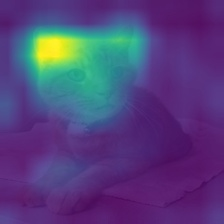
\includegraphics[scale=0.5]{img/cat1.jpg}
    \end{minipage}
    \begin{minipage}{0.25\textwidth}
        \centering
        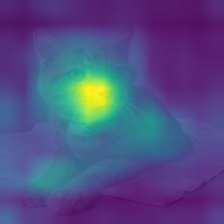
\includegraphics[scale=0.5]{img/cat2.jpg}
    \end{minipage}
    \begin{minipage}{0.25\textwidth}
        \centering
        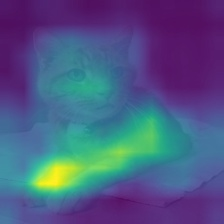
\includegraphics[scale=0.5]{img/cat3.jpg}
    \end{minipage}
    \caption{cat的热力图}
\end{figure}
\begin{figure}[htbp]
    \centering
    \begin{minipage}{0.25\textwidth}
        \centering
        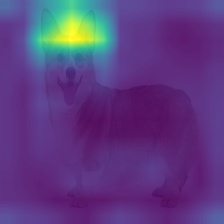
\includegraphics[scale=0.5]{img/dog1.jpg}
    \end{minipage}
    \begin{minipage}{0.25\textwidth}
        \centering
        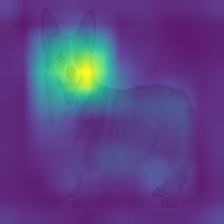
\includegraphics[scale=0.5]{img/dog2.jpg}
    \end{minipage}
    \begin{minipage}{0.25\textwidth}
        \centering
        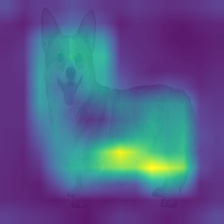
\includegraphics[scale=0.5]{img/dog3.jpg}
    \end{minipage}
    \caption{dog的热力图}
\end{figure}
\begin{figure}[htbp]
    \centering
    \begin{minipage}{0.25\textwidth}
        \centering
        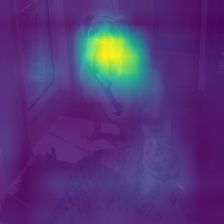
\includegraphics[scale=0.5]{img/both1.jpg}
    \end{minipage}
    \begin{minipage}{0.25\textwidth}
        \centering
        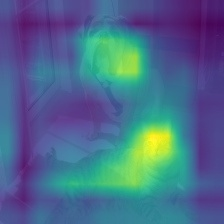
\includegraphics[scale=0.5]{img/both2.jpg}
    \end{minipage}
    \begin{minipage}{0.25\textwidth}
        \centering
        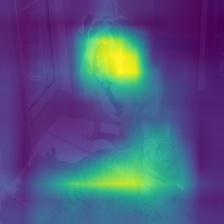
\includegraphics[scale=0.5]{img/both3.jpg}
    \end{minipage}
    \caption{both的热力图}
\end{figure}

某些通道的热力图可能显示出对猫和狗耳朵的高关注度。这表明模型在区分猫和狗时认为耳朵是重要的特征。耳朵的形状、大小、位置等特征可能对模型的分类决策起到一定的作用。

某些通道的热力图可能显示出对猫和狗身体的高关注度。这表明模型可能将身体的特征视为区分猫和狗的重要依据。身体的形状、纹理、颜色等特征可能在模型的分类决策中扮演关键角色。

某些通道的热力图可能显示出对猫和狗面部的高关注度。这可以解释为什么模型能够正确识别猫和狗,因为它们的面部通常具有明显的特征差异。例如,猫和狗的眼睛、鼻子、嘴巴等部位可能在模型的决策中起到重要作用。

当猫和狗同时出现在一张图片中时,模型可能会专注于它们的面部和身体。这是因为猫和狗的面部和身体通常是它们的重要特征,能够帮助区分它们的类别。模型可能会通过学习猫和狗的面部特征(如眼睛、鼻子、口部)以及身体形态(如身体轮廓、四肢位置)来对它们进行区分。

这种观察结果进一步证明了Grad-CAM方法的有效性。通过生成热力图,我们可以直观地观察到模型对于不同类别的关注区域,从而理解模型在决策过程中的注意力分布。在这个案例中,我们可以看到模型对于猫和狗的不同部位有明显的关注,这与我们对于猫和狗的视觉感知和区分有一定的一致性。
\chapter{总结}
通过本次实验,我们使用了Grad-CAM和LayerCAM这两种可解释性技术,对卷积神经网络(CNN)的注意力分布进行了可视化,并专注于研究猫和狗图像分类任务。以下是我在实验过程中的一些心得体会:
\begin{enumerate}
\item 可解释性的重要性:对于深度学习模型而言,可解释性是一个重要的研究领域。通过了解模型关注的区域和特征,我们可以更好地理解模型的决策过程,并验证模型是否根据我们期望的特征进行分类。

\item Grad-CAM和LayerCAM的应用:Grad-CAM和LayerCAM是两种流行的可解释性技术,通过生成热力图可视化模型的注意力分布。这些技术能够帮助我们定位模型关注的区域,发现模型用于分类的关键特征。

\item 观察结果的解读:在实验中,观察到模型在猫和狗同时存在的图像中,更多地关注它们的面部和身体部位。这符合我们的直观认知,因为面部和身体特征对于猫和狗的识别是非常重要的。

\item 模型的学习能力:通过观察模型的注意力分布,我们可以发现模型学习到了与不同类别相关的特征。模型能够自动关注这些特征,并基于它们进行分类决策,这体现了模型在学习任务中的有效性。
\end{enumerate}

总之,通过可解释性技术的应用,我们能够更好地理解CNN模型的决策过程,并验证模型是否根据我们期望的特征进行分类。这些技术为深度学习模型的可解释性提供了有力的工具,对于进一步探索和改进模型性能具有重要意义。
\end{document}
\endinput
%%
%% End of file `hustreport-zh-example.tex'.
